\documentclass[12pt, a4paper, oneside]{ctexart}
\usepackage{amsmath, amsthm, amssymb, graphicx}
\usepackage{hyperref}
\usepackage{listings}
\usepackage{xcolor}
\usepackage{color}
\usepackage{enumerate}
\usepackage{epstopdf}
\usepackage{float}
\usepackage{booktabs}
\hypersetup{
    colorlinks=true,
    linkcolor=blue,
    filecolor=blue,      
    urlcolor=blue,
    citecolor=cyan,
}
\definecolor{dkgreen}{rgb}{0,0.6,0}
\definecolor{gray}{rgb}{0.5,0.5,0.5}
\definecolor{mauve}{rgb}{0.58,0,0.82}

\lstset{ %
    language=Python,                % the language of the code
    basicstyle=\footnotesize,           % the size of the fonts that are used for the code
    numbers=left,                   % where to put the line-numbers
    %numberstyle=\tiny\color{gray},  % the style that is used for the line-numbers
    %stepnumber=2,                   % the step between two line-numbers. If it's 1, each line 
                            % will be numbered
    %numbersep=5pt,                  % how far the line-numbers are from the code
    %backgroundcolor=\color{blue},      % choose the background color. You must add \usepackage{color}
    showspaces=false,               % show spaces adding particular underscores
    %showstringspaces=false,         % underline spaces within strings
    showtabs=false,                 % show tabs within strings adding particular underscores
    frame=single,                   % adds a frame around the code
    rulecolor=\color{black},        % if not set, the frame-color may be changed on line-breaks within not-black text (e.g. commens (green here))
    tabsize=2,                      % sets default tabsize to 2 spaces
    captionpos=b,                   % sets the caption-position to bottom
    breaklines=true,                % sets automatic line breaking
    breakatwhitespace=false,        % sets if automatic breaks should only happen at whitespace
    title=\lstname,                   % show the filename of files included with \lstinputlisting;
                            % also try caption instead of title
    keywordstyle=\color{blue},          % keyword style
    commentstyle=\color{dkgreen},       % comment style
    stringstyle=\color{mauve},         % string literal style
    escapeinside={\%*}{*)},            % if you want to add LaTeX within your code
    morekeywords={*,...}               % if you want to add more keywords to the set
}
\title{动态规划解决邮筒安排问题}
\author{Xiaoma}
\date{\today}
\begin{document}
\maketitle
\section{问题描述}
\begin{itemize}
    \item 假设在一条街道上散布着若干房屋$houses$,即此时将街道视作一条直线,而房屋为直线上的若干个点,现在需要在这条街道上安装
    $k$个邮筒,邮筒安装位置应保证每栋房子到邮筒的距离尽可能近,为了兼顾用户体验与安装成本,现在需要计算不同邮筒数量对应的每栋房子与离它最近
    的邮筒之间的距离的最小的总和。
    \item 假设数组$houses$中的值为房屋的位置
    例如
    \begin{figure}[H]
        \centering
        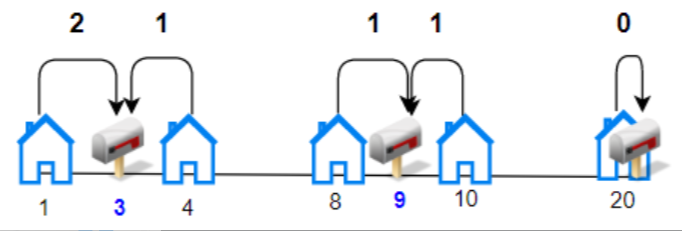
\includegraphics[scale=0.6]{1.png}
    \end{figure}
    $houses$中的值分别为$"1, 4, 8, 10, 20"$,邮筒的数量$k = 3$。\\
    将邮筒分别安排在位置$3,9,20$处,得到在该情况下每个房子与最近的邮筒的距离的和为$5$。
\end{itemize}
\section{算法原理}
\subsection{动态规划}
动态规划在数学上属于运筹学的一个分支,是求解决策过程最优化的数学方法
,同时也是计算机科学领域中一种常见的算法思想。

动态规划算法与我们前面提及的分治算法相似,
都是通过组合子问题的解来求解原问题的解。
但是两者之间也有很大区别:
分治法将问题划分为互不相交的子问题,
递归的求解子问题,
再将他们的解组合起来求解原问题的解;
与之相反,
动态规划应用于子问题相互重叠的情况,
在这种情况下,
分治法还是会做很多重复的不必要的工作,
他会反复求解那些公共的子问题,
而动态规划算法则对相同的每个子问题只会求解一次,
将其结果保存起来,避免一些不必要的计算工作。

动态规划算法更多的时候是用来求解一些最优化问题,
这些问题有很多可行解,每个解都有一个值,
利用动态规划算法是希望找到具有最优值的解。

\subsubsection{动态规划的适用条件}
\begin{itemize}
    \item 最优子结构:利用动态规划算法求解问题的第一步需要寻找问题最优解的
    结构,如果一个问题的最优解包含其子问题的最优解,则次问题具备最优子结构的性质。
    \item 重叠子问题:即原问题递归求解时会重复相同的子问题,而不是一直生成子问题。
\end{itemize}

\subsection{解题思路}
当且仅当某个邮筒是距离某房子最近的邮筒时,该邮筒负责该房子,对任意一个邮筒
,其负责的房子的集合在数轴上是连续的。因此首先应将$houses$数组进行排序然后再
安排邮筒。

假设在只有一个邮筒的情况下,若邮筒安排在数组$houses$的中位数的位置,可以得到最小距离总和。

证明:

设数组$houses$包含$n$个元素,且其互不相同,证明当$x = median(houses)$时,有
$$
\sum_{i=1}^{n}| houses[i] - x\vert \leq \sum_{i=1}^{n}| houses[i] - y\vert \quad (y \in \mathbb{R})
$$
成立。

将数组$houses$进行升序排列,并补充$houses[0] = -\infty $,$houses[n+1] = \infty$,记
$$
f(x) = \sum_{i=1}^{n}| houses[i] - x\vert
$$
对$f(x)$求导,得
$$
f'(x) = \sum_{i=1}^{n} \mathbb{I}(houses[i])
$$
已知$houses$有序,则$\exists i_{0} \in [0, n+1),s.t. \ houses[i_{0}] \leq x < houses[i_{0} + 1]$。
\begin{itemize}
    \item 如果$houses[i] < x < houses[i_{0} + 1]$,
    $$f'(x) = \sum_{i = 1}^{i_{0}}1 + \sum_{i = i_{0} + 1}^{n}(-1)=2i_{0} - n$$
    \item 如果$houses[i] = x$,则$f(x)$在该点连续但不可导。
\end{itemize}
若想要寻找$f(x)$的最小值,只需要关注$f'(x)$的正负性。已知
$$
f'(x) = 2i_{0} - n
$$
当$i_{0} \leq \lfloor (n-1)/2\rfloor $时,$f'(x) < 0$,此时$f(x)$单调递减。同理可得
,当$i_{0} \geq \lceil (n+1)/2\rceil $时,$f'(x) > 0$,此时$f(x)$单调递增。

\begin{itemize}
    \item 当$n$为奇数时,$\lfloor (n+1)/2\rfloor=\lceil (n+1)/2\rceil=(n+1)/2$,$f(x)$在$houses[(n+1)/2]$处取得最小值,
    对应了数组$houses$的中位数
    \item 当$n$为偶数时,$\lfloor (n+1)/2\rfloor=n/2,\lceil (n+1)/2\rceil=n/2 + 1$,$f(x)$在$x \in houses[n/2], houses[n/2+1]$
    处取得最小值,对应了数组$houses$的中位数
\end{itemize}

使用$f[i][j]$来表示前$i$栋房子(从0开始编号)安排$j$个邮箱的最小距离总和。在进行状态转移时,可以
枚举第$j$个邮筒负责的房子的起始编号,从$i_{0}+1$开始,到$i$结束,得到的状态转移方程为
$$
f[i][j] = min(f[i_{0}][j - 1] + cost(i_{0} + 1, i))
$$
以及边界条件
$$
f[i][1] = cost(0,i)
$$
其中$cost(l,r)$表示给排好序的$houses[l]$到$houses[r]$的房子安排一个邮筒,可以得到的最小距离总和。
而其结果就是最开始证明的,当邮箱位置在$houses$中位数时,$houses[l]$到$houses[r]$的房子与其距离的和。

另外,在状态转移方程中,有一些状态是无意义的,对于$f[i][j]$,当$j > i$即邮筒的数量大于房子的数量时,
结果显然没有意义,故不需要额外计算。

\section{数据集说明}
假设任意邮筒数量(合理值)

使用生成随机数的方法生成了房子的位置
\begin{lstlisting}
    20
    1 5 8 9 6 4 7 25 36 98 65 74 12 22 55 88 77 20 60 47 84 152 112 135 99 105 107 103 120
\end{lstlisting}

只列出一种输入值,其他情况不再赘述

\section*{程序输入输出说明}
运行该程序以后,需要进行两段输入,首先输入需要安排的邮筒数,然后输入房子的位置,数字间用空格分隔。

程序最后输出每栋房子到与其最近的邮筒的距离的和,以及算法运行时间。

\section{程序测试结果}
\begin{figure}[H]
    \centering
    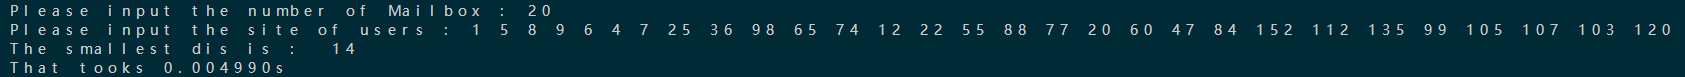
\includegraphics[scale=0.3]{2.png}
\end{figure}
\section{分析总结}
实验实现了对邮筒安排问题用户成本的计算,该算法也可适用于其他类似的现实问题,
相对来说较为贴近现实生活,在理论计算的过程中较为繁琐,但代码实现较为简单。
\end{document}

